\documentclass[a4paper,landscape]{amsart}
\usepackage[top=1cm,bottom=1cm,left=0.75cm,right=0.75cm]{geometry}
\usepackage{siunitx}
\usepackage{tikz}
\usetikzlibrary{calc}
\usepackage{pgfplots}
\pgfplotsset{compat=1.3}

\begin{document}
	\thispagestyle{empty}
	\begin{figure}
		\centering
		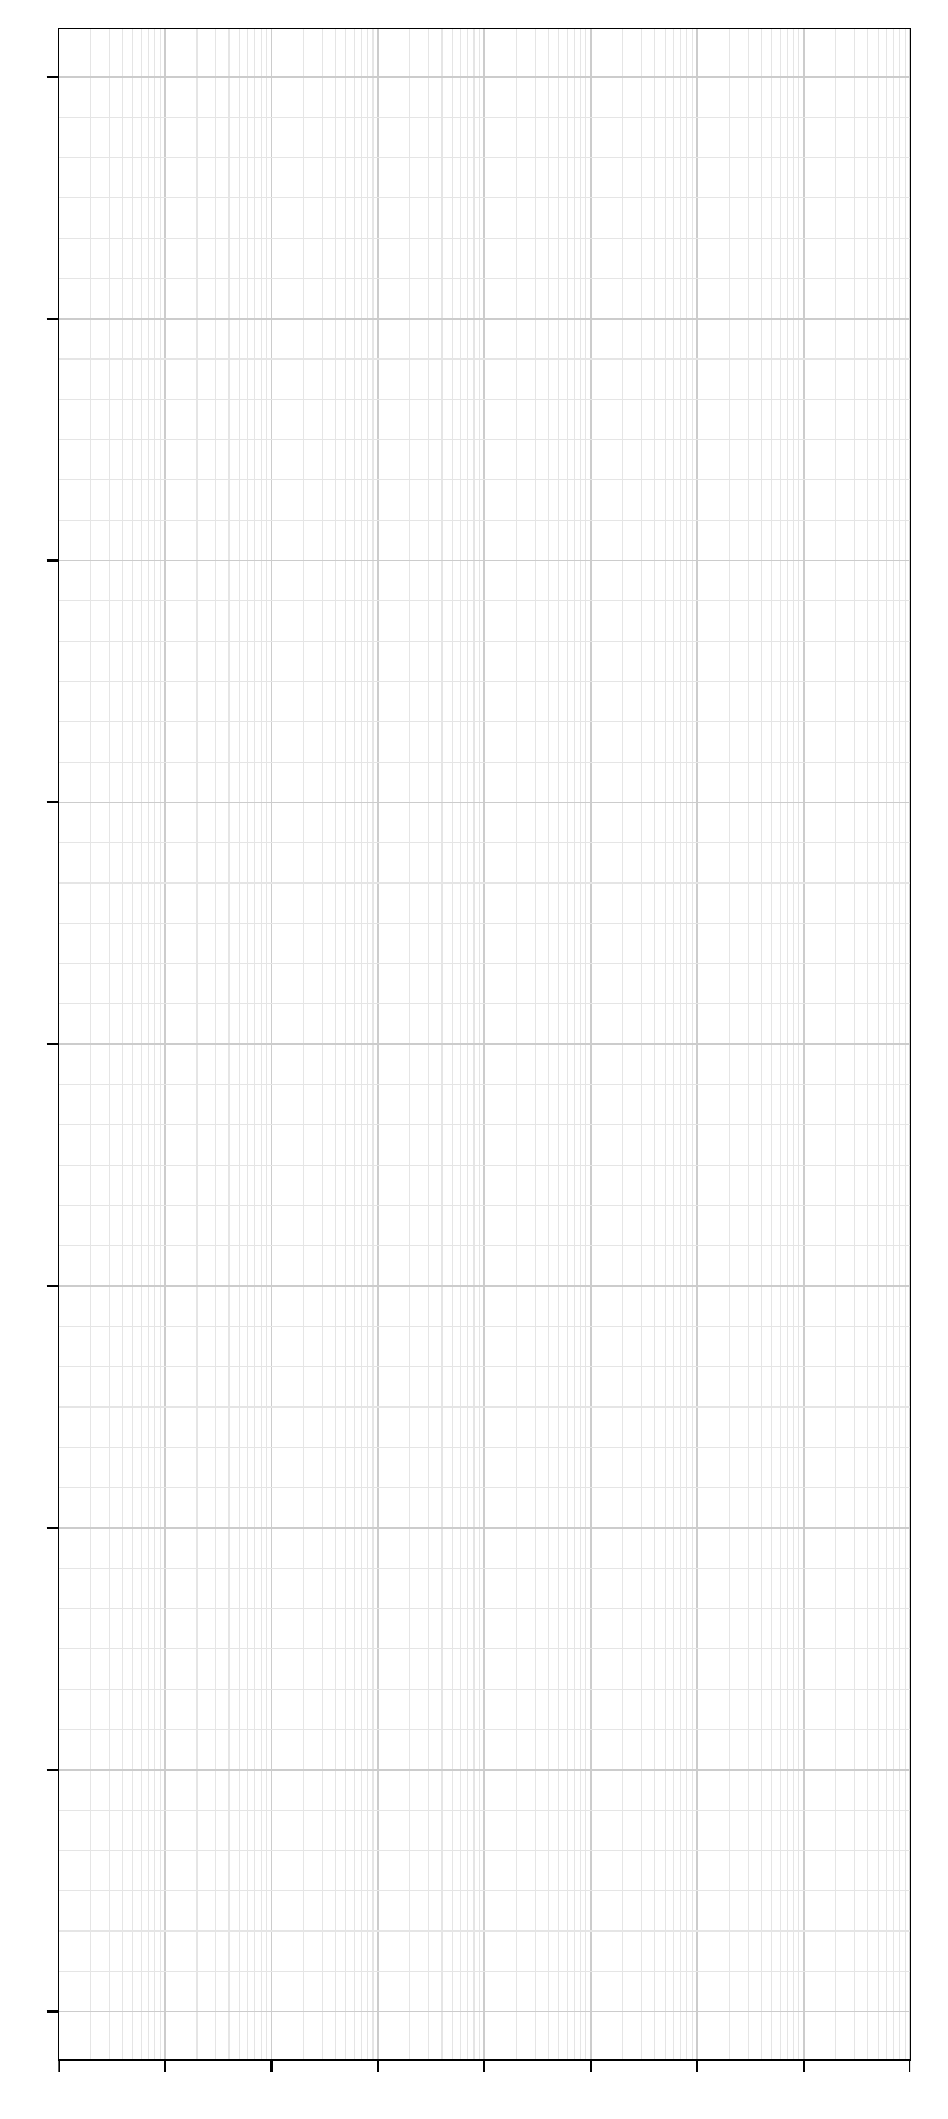
\begin{tikzpicture}
		\begin{axis}[
		name=magnitude,
		%title={\texttt{\large{Magnitude}}},
		width=1.0225\linewidth,
		height=0.98\paperheight,
		xmode=log,
		ymode=linear,
		axis line style={latex-latex},
		%xlabel={$\omega$[\si[per-mode=fraction]{\radian\per\second}]},
		xlabel style={at={(ticklabel* cs:1,8)},anchor=north},
		%ylabel={\si{\decibel}},
		ylabel style={rotate=-90,at={(ticklabel* cs:1)},anchor=south},
		xmin=1e-4,xmax=1e4,
		ymin=-60,ymax=100,
		enlarge y limits=0.025,
		ytick align=outside,
		xtick align=outside,
		ytick pos=left,
		xtick pos=left,
		minor tick length=0pt,
		ytick={-60,-40,...,100},
		yticklabels={},
		xticklabels={},
		%ytick={-60,-40,...,100},
		grid=both,
		minor tick num=5,
		grid style={line width=.4pt, draw=gray!20},
		minor tick style={line width=.4pt, draw=gray!20},
		major tick style={line width=.8pt,draw=black},
		major grid style={line width=.6pt,draw=gray!40},
		ticklabel style={font=\footnotesize}
		]
		%\addplot[mark=none,line width=.8pt,gray!80,domain=0.011:9000]{0}; % Makes "0 axis" thicker
		\end{axis}
		%\node[above,font=\large\bfseries] at ($(magnitude.north)+(0,1)$) {\texttt{\LARGE{Semilog Paper}}};
		\end{tikzpicture}		
	\end{figure}
\end{document}